\documentclass[11pt,a4paper,xcolor=table, handout]{beamer} % ,handout: for printing
\usepackage{etex}
%\documentclass[handout]{beamer}

\usetheme{Madrid}

%
% To use when printing
%
\iffalse
\usepackage{pgfpages}
\mode<handout>{
  \usetheme{default}
  \setbeamercolor{}{bg=black!5} % \setbeamercolor{background canvas}{bg=black!5} 
  \pgfpagesuselayout{4 on 1}[letterpaper,landscape,border shrink=2.5mm]
}
\fi

\usepackage[utf8]{inputenc} % [utf8] for linux, latin1 for windows
\usepackage[french]{babel}
%\usepackage{fullpage}
\usepackage{amsmath}
\usepackage{amsfonts}
\usepackage{amssymb}
\usepackage{graphicx} 
\usepackage{longtable}
\usepackage{algorithm}
\usepackage{listings}
\usepackage{algorithmic}
\usepackage{float}

\usepackage[center]{caption}
\usepackage{subcaption}

\usepackage[table]{xcolor}

\definecolor{colorperso}{RGB}{165,165,165}
%\usepackage[utf8]{inputenc}
%\usepackage[francais]{babel}
%\usepackage[T1]{fontenc}

%\usepackage{amsmath}
%\usepackage{amsfonts}
%\usepackage{amssymb}

%\usepackage{amsthm}
%\usepackage{graphicx}

\usepackage{tikz,pgfplots}
\usepackage[all]{xy}

% tikz stuff
\usetikzlibrary{shapes,arrows,decorations.pathreplacing, calc, intersections}
\makeatletter
\newcommand{\gettikzxy}[3]{%
  \tikz@scan@one@point\pgfutil@firstofone#1\relax
  \edef#2{\the\pgf@x}%
  \edef#3{\the\pgf@y}%
}
\makeatother

\newtheorem*{mydef}{Definition}
%\newtheorem*{definition}{Definition}
\newtheorem{mythm}{Theorem}
\newtheorem{requirement}{Requirement}
\newtheorem*{mynot}{Notation}
\newtheorem{myprop}{Proposition}

\newcommand{\var}{\operatorname{Var}}
\newcommand{\Bequal}{\mathrel{\widehat{=}}}
\def\p#1{\mathrel{\ooalign{\hfil$\mapstochar\mkern 5mu$\hfil\cr$#1$}}}
\def\f#1{\mathrel{\ooalign{\hfil
    $\mapstochar\mkern 3mu\mapstochar\mkern 5mu$\hfil\cr$#1$}}}
\def \pfun  {\p\rightarrow}

\makeatother
\setbeamertemplate{footline}
{
  \leavevmode%
  \hbox{%
  \begin{beamercolorbox}[wd=.4\paperwidth,ht=2.25ex,dp=1ex,center]{author in head/foot}%
    \usebeamerfont{author in head/foot}\insertshortauthor
  \end{beamercolorbox}%
  \begin{beamercolorbox}[wd=.6\paperwidth,ht=2.25ex,dp=1ex,center]{title in head/foot}%
    \usebeamerfont{title in head/foot}\insertshorttitle\hspace*{3em}
    \insertframenumber{} / \inserttotalframenumber\hspace*{1ex}
  \end{beamercolorbox}}%
  \vskip0pt%
}
\makeatletter

\setbeamertemplate{navigation symbols}{}

\author[]{Jean-Baptiste Lespiau}
\author{Jean-Baptiste Lespiau et Charles Thin}
\title{La méthode B : une méthode formelle de développement logiciel}
\date\today

\begin{document}

\frame{\titlepage}

\section*{Introduction}

\begin{frame}
\frametitle{Introduction}
\framesubtitle{Qu'est-ce que la méthode B ?}
\begin{figure}[h]

\includegraphics[scale=0.2]{ressources/logo1.png}
\end{figure}
La méthode B, inventée par Jean-Raymond Abrial, c'est :\\~\\
\begin{itemize}
\item Un langage (le langage B)\\~\\
\pause
\item Un outil (l'Atelier B)\\~\\
\pause
\item Une méthode (la méthode B)
\end{itemize}
\end{frame}

\begin{frame}
\frametitle{Introduction}
\framesubtitle{À quoi sert le langage B ?}
B est un langage unique pour :\\~\\
\pause
\begin{itemize}
\item Spécifier formellement des fonctionnalités du logiciel
\pause
\item Spécifier formellement des propriétés du logiciel
\pause
\end{itemize}
~\\
Et ce à tout niveau d'abstraction.
\end{frame}

\begin{frame}
\frametitle{Introduction}
\framesubtitle{À quoi sert l'Atelier B ?}
\begin{figure}[h]
\centering

\includegraphics[scale=0.2]{ressources/logo.png}
\end{figure}
\pause
L'Atelier B (ClearSy) est l'outil principal où l'on écrit du B et où on le vérifie. Il est donc au coeur de la méthode B.\\~\\
\pause
Il comprend :
\begin{itemize}
\item un analyseur
\pause
\item un générateur d'obligation de preuve
\pause
\item un démonstrateur automatique
\pause
\item un démonstrateur interactif
\pause
\item un générateur de code C et Ada
\pause
\item un gestionnaire de projet...
\end{itemize}
\end{frame}

\begin{frame}
\frametitle{Introduction}
\framesubtitle{À quoi sert ... la méthode B ?}
La méthode B, enfin, encadre le processus industriel.\\~\\ \pause
C'est une méthode formelle par laquelle on peut :\pause
\begin{itemize}
\item Énoncer en B les fonctionnalité du logiciel en développement
\pause
\item Les raffiner (concrétiser) jusqu'à obtenir une implémentation
\pause
\end{itemize}
Et en même temps :\pause
\begin{itemize}
\item Énoncer en B des propriétés sur le logiciel en développement
\pause
\item Les vérifier lors du développement (du raffinement) dans l'Atelier B
\pause
\end{itemize}
Pour enfin :
\begin{itemize}
\item Générer du code fonctionnel (en un langage compilable ``classique'') ...
\pause
\item ... qui vérifie par construction les propriétés voulues !
\end{itemize}
\end{frame}

%
% Plan
%
\frame{\tableofcontents}

\section{Modélisation formelle}
\subsection{Théorie des ensembles}
\begin{frame}
\frametitle{Modélisation formelle}
\framesubtitle{Théorie des ensembles}
Pour spécifier formellement des propriétés, on utilise la théorie des ensembles dans le cadre ZFC.
\\~\pause
\begin{description}
\item[Définition de la paire] $(E, F) \in s \times t \Leftrightarrow E \in s \wedge F \in t$
\item[Ensemble des parties] $s \in \mathbb{P}(t) \Leftrightarrow \forall x (x \in s \Rightarrow x \in t)$
\item[Ensemble en compréhension] $E \in \{ x | x \in s \wedge P \} \Leftrightarrow (E \in s \wedge [x:= E] P)$
\item[Égalité d'ensembles] $\forall x (x \in s \Leftrightarrow x \in t) \Rightarrow s = t$
\item[Axiome du choix] $\exists x  (x \in s) \Rightarrow choice(s) \in s$
\item[Axiome de l'infini] Existence d'un ensemble infini nommé BIG
\end{description}
\end{frame}

\subsection{Substitutions généralisées}
\begin{frame}
\frametitle{Modélisation formelle}
\framesubtitle{Logique de Hoare et substitutions généralisées}
\begin{definition}
$ \{P\}\;S\;\{Q\} $ : si la propriété $P$ est vraie et qu'on exécute le code $S$, alors si $S$ termine on a la propriété $Q$.
\end{definition}

Pour spécifier formellement des opérations, on utilise les substitutions généralisées.
\\\pause
Une substitution remplace des éléments par des expressions dans une propriété :\\[5pt]
[x := E](A $\wedge$ x) $\Leftrightarrow$ A $\wedge$ E\\[5pt]
[n := n+1](n $\leq$ max) (itération de boucle)
\\[10pt]\pause
Si l'on veut s'assurer qu'une propriété P est vérifiée après avoir appliqué une substitution S, il faut qu'avant l'application de S, une précondition minimale soit vérifiée, notée [S]P.\pause Par exemple :\\[5pt]
[n := n+1](n $\leq$ max) $\Leftrightarrow$ n $\leq$ max\ -\ 1\pause\\
[n := n+1](n $\leq$ max $\wedge$ n $\in$ $\mathbb{N}$) $\Leftrightarrow$ n $<$ max
\end{frame}


\iffalse
\begin{frame}
\frametitle{Ce qu'il faut retenir}
\begin{itemize}
\item B est un langage et une méthode de spécification
\item C'est une méthode formelle (permettant des preuves)
\item Le langage est basé sur la théorie des ensembles
\item Une spécification simple est une machine abstraite
\item Une machine abstraite décrit :
\begin{itemize}
\item L'état du système modélisé (variables typées)
\item Certaines de ses propriétés (invariant)
\item Les services qu'il offre (opérations)
\end{itemize}
\item La vérification (preuve) assure que les services satisfont les
propriétés
\item Les preuves démontrent la préservation d'un invariant
\item Les preuves s'effectuent par calcul des plus faibles préconditions
(calcul des substitutions)
\end{itemize}
\end{frame}
\fi

\section{Modélisation en B}
\subsection{Généralités}
\begin{frame}
\frametitle{Modélisation en B}
\framesubtitle{Généralités}
On \emph{modélise} un futur logiciel ou un système en B avec des machines abstraites.\\[5pt]~\pause
Ces machines spécifient\pause
\begin{itemize}
\item des propriétés (potentiellement abstraites)
\pause
\item des opérations (qui conservent ces propriétés).
\pause
\end{itemize}
~\\[0pt]
La correction des opérations (les \emph{obligations de preuves}) est vérifiée dans l'Atelier B à l'aide du démonstrateur.\pause\\[5pt]
Ces machines peuvent être concrétisées (on dit: \emph{raffinées}) jusqu'à une \emph{implémentation}.
\end{frame}

\subsection{Les machines abstraites}
\begin{frame}
\frametitle{Les machines abstraites}
\framesubtitle{Éléments}
Une machine abstraite spécifie au moins :
\begin{itemize}
\pause
\item Un nom
\pause
\item Des ensembles de travail
\pause
\item Des constantes et variables
\pause
\item Des propriétés et invariants
\pause
\item Des opérations
\end{itemize}
\end{frame}

\begin{frame}
\frametitle{Les machines abstraites}
\framesubtitle{Un exemple}
Spécifions une bibliothèque où il y a des livres (concept abstrait), des exemplaires, et des abonnés.\\\iffalse\fi\pause
On peut créer un nouveau livre, \pause en emprunter un exemplaire, \pause et en rendre un.
\\\iffalse\fi\pause Seuls les abonnés ont accès à ces services.
\\\iffalse\fi\pause Il peut y avoir plusieurs exemplaires d'un même livre.
\\\iffalse\fi\pause Il y a une limite au nombre d'emprunts par abonné.
\\~\\\iffalse\fi\pause Ceci est une spécification en langage naturel.
\end{frame}

\begin{frame}
\frametitle{Les machines abstraites}
\framesubtitle{Un exemple}
\setlength{\LTpre}{\medskipamount}
\setlength{\LTpost}{0pt}
\setlength\LTleft{\parindent}
\textbf{MACHINE}  BIBLIOTHEQUE (maxi) \\
\noindent\textbf{CONSTRAINTS} maxi $\in$ N1 \\
\noindent\textbf{SETS}
\begin{longtable}{ll} LIVRES; \\ PERSONNES\\ \end{longtable}
\noindent\textbf{VARIABLES}
\begin{longtable}{ll} livre , exemplaire , abonne , emprunt \end{longtable}
\noindent\textbf{INVARIANTS}
\begin{longtable}{ll}
$livre \subseteq LIVRE $ & $\wedge$ \tabularnewline
$abonne \subseteq PERSONNE$ & $\wedge$ \tabularnewline
$exemplaire \in livre \leftrightarrow N1$ & $\wedge$ \tabularnewline
$emprunt \in ( exemplaire \pfun abonne )$ & $\wedge$ \tabularnewline
$\forall ab\ (\ ab \in abonne \Rightarrow (\ \textbf{card}\ (\ emprunt ^{-1}\{ab\} \leq maxi\ ))$ &
\end{longtable}
\end{frame}

\begin{frame}
\frametitle{Les machines abstraites}
\framesubtitle{Un exemple}
\noindent\textbf{INITIALISATION}
\begin{longtable}{ll}
$livre := \{Oui-Oui,\ Comment\ Mourir,\ Le\ Code\ Civil\} $& $||$ \tabularnewline
$exemplaire := \{1 \mapsto Oui-Oui,\ 2 \mapsto Oui-Oui,\ 1 \mapsto Comment\ Mourir\}$ & $||$ \tabularnewline
$abonne := \{Jean\ Dupont,\ Blob\ Duchmol,\ Pierre\ Smash\} $& $||$ \tabularnewline
$emprunt := \{Pierre\ Smash \mapsto ( 2 \mapsto Oui-Oui)\ \}$ &
\end{longtable}
\end{frame}

\begin{frame}
\frametitle{Les machines abstraites}
\framesubtitle{Un exemple}
\noindent \textbf{OPERATIONS}

~\\
\indent lr $\leftarrow$ creer\_Livre $\Bequal$

\textbf{PRE} LIVRE - livre $\neq$ $\emptyset$ \textbf{THEN}

\hspace*{1em} \textbf{ANY} $ll$ \textbf{WHERE}  \emph{ll} $\in$ LIVRE - livre \textbf{THEN} 

\hspace*{2em}  livre := livre $\cup$ \{$ll$\} $||$ 

\hspace*{2em} lr := $ll$

\hspace*{1em} \textbf{END}

\textbf{END};

\end{frame}

\begin{frame}
\frametitle{Les machines abstraites}
\framesubtitle{Un exemple}
\indent emprunter(\emph{aa}, \emph{ll}) $\Bequal$
\begin{longtable}{lll}
\textbf{PRE} \tabularnewline
~~~~ \emph{aa} $\in$ abonne & $\wedge$ \tabularnewline 
~~~~ \emph{ll} $\in$ livre & $\wedge$ \tabularnewline
~~~~ $\exists$ \emph{nn}.\ (\emph{nn} $\in$ N1 $\wedge$ \emph{ll} $\mapsto$ \emph{nn} $\in$ exemplaire $\wedge$ \emph{ll} $\mapsto$ \emph{nn} $\notin$ dom(emprunt)) & $\wedge$ \tabularnewline
~~~~ \textbf{card}(emprunt $^{-1}$[$\{$ab$\}$] $<$ maxi) \tabularnewline
\textbf{THEN} \tabularnewline ~~~~ emprunt := emprunt $\cup$ \{(\emph{ll} $\mapsto$ \emph{nn}) $\mapsto$ \emph{aa})\} \tabularnewline
\textbf{END} \tabularnewline
\end{longtable}
\end{frame}

\begin{frame}
\frametitle{Les machines abstraites}
\framesubtitle{Un exemple}
\indent retourner(\emph{aa}, \emph{ll}) $\Bequal$
\begin{longtable}{lll}
\textbf{PRE} \tabularnewline
~~~~ \emph{aa} $\in$ abonne & $\wedge$ \tabularnewline 
~~~~ \emph{ll} $\in$ livre & $\wedge$ \tabularnewline
~~~~ $\exists$ \emph{nn}.\ (\emph{nn} $\in$ N1 $\wedge$ \emph{ll} $\mapsto$ \emph{nn} $\in$ exemplaire $\wedge$ (\emph{ll} $\mapsto$ \emph{nn}) $\mapsto$ \emph{aa} $\in$ emprunt )\tabularnewline
\textbf{THEN} \tabularnewline
~~~~ \textbf{ANY} \emph{nn} \textbf{WHERE} \tabularnewline
~~~~ ~~~~ \emph{nn} $\in$ N1 $\wedge~ll \mapsto$ \emph{nn} $\in$ exemplaire & $\wedge$ \tabularnewline
~~~~ ~~~~ (\emph{ll} $\mapsto$ \emph{nn}) $\mapsto$ \emph{aa} $\in$ emprunt \tabularnewline
~~~~ \textbf{THEN} \tabularnewline
~~~~ ~~~~ emprunt := emprunt -- \{(\emph{ll} $\mapsto$ \emph{nn}) $\mapsto$ \emph{aa})\} \tabularnewline
\textbf{END} \tabularnewline
\end{longtable}
\end{frame}

\subsection{Le raffinement de machines}
\begin{frame}
\frametitle{Le raffinement de machines}
\framesubtitle{Les bases}
Le raffinement est le fait de transformer une spécification abstraite en un texte plus proche de la programmation, pour finalement obtenir un programme.

En pratique il s'agit de :
\begin{itemize}
\pause
\item Reformuler en fonction du changement d'état
\pause
\item Affaiblir des préconditions
\pause
\item Concrétiser les ensembles
\pause
\item Réduire le non-déterminisme
\end{itemize}
\pause
Tout en gardant bien sûr les invariants au long des opérations. Or on a modifié les opérations, en les remplaçant par des raffinements : ainsi, il faut que les invariants et les éventuelles préconditions impliquent la plus petite précondition des nouvelles substitiutions, telles qu'à la fin les invariants soient encore vérifiés.
\end{frame}

\begin{frame}
\frametitle{Le raffinement de machines}
\framesubtitle{Les bases}
\begin{figure}[h]
\centering
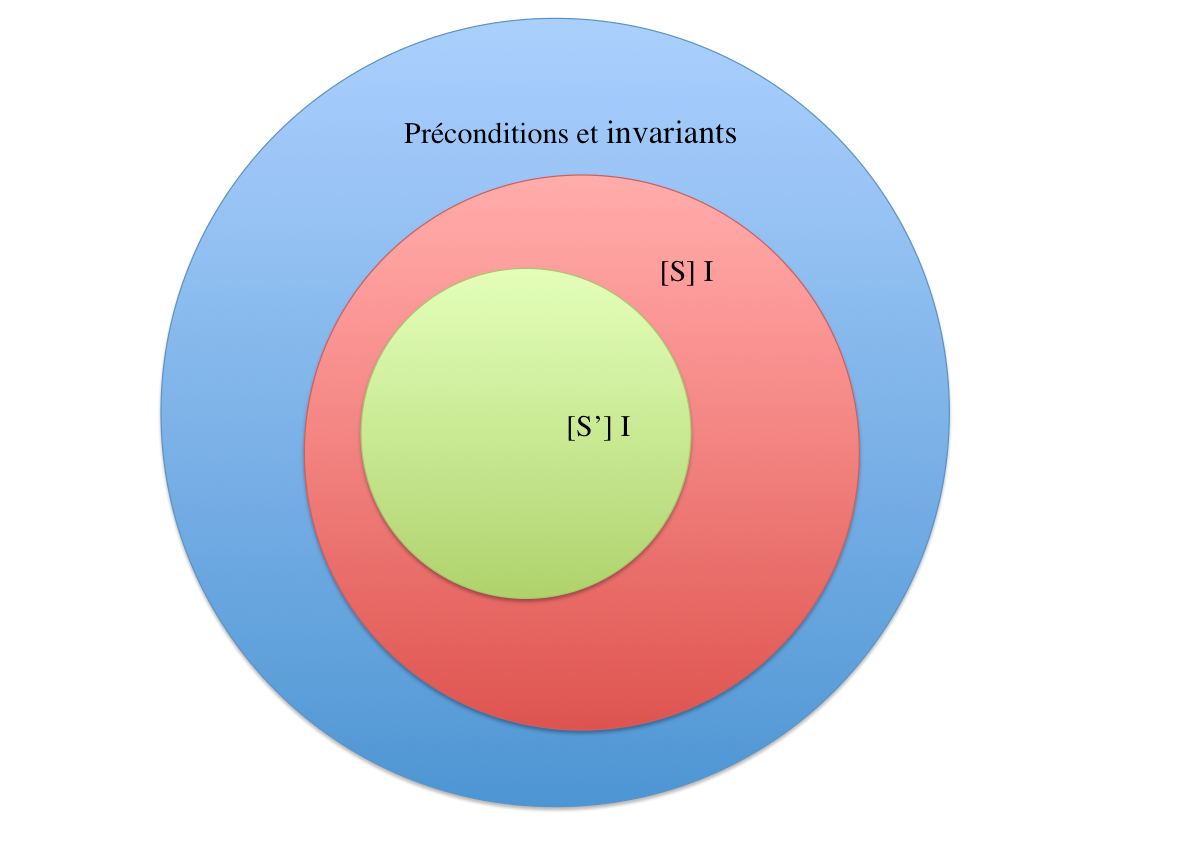
\includegraphics[scale=0.25]{ressources/cond.png}
\end{figure}
\end{frame}

\subsection{L'implémentation}
\begin{frame}
\frametitle{Implémentations}
Le langage $B_0$ est un sous langage de la méthode B qui est directement traduisible en un programme (en ADA, C, C++, etc.).  Il est ainsi très proche d'un langage séquentiel.

\pause

On impose un certain nombre de restrictions :
\begin{itemize}
\item aucune précondition
\pause
\item que des substitutions déterministes ( $:=$, \textsc{IF}, ";" par exemple, mais pas de choix)
\pause
\item toutes les constantes et variables sont d'un type concret
\pause
\item la terminaison et la correction des boucles doit être prouvée par l'utilisation d'invariants et de variants
\end{itemize}
~\\~\\\pause
La phase finale de la méthode B consiste en la génération de code.

\end{frame}

\begin{frame}
\frametitle{Le raffinement des machines}
\framesubtitle{Un exemple simple}
\noindent \textbf{MACHINE} utils \\
\textbf{CONSTANTS} $t,n$ \\
\textbf{OPERATIONS} \\
$res \leftarrow mini(x, y) \Bequal$ \\
\hspace*{1em}  \textbf{PRE} $x \in \mathbb{N} \wedge  y \in \mathbb{N} $ \textbf{THEN} \\
\hspace*{2em} res := min(\{x, y\})  \\
\hspace*{1em} \textbf{END} \\
$res \leftarrow maxi(x, y, z) \Bequal$ \\
\hspace*{1em}  \textbf{PRE} $x \in \mathbb{N} \wedge  y \in \mathbb{N} \wedge z \in \mathbb{N}$ \textbf{THEN} \\
\hspace*{2em} res := max(\{x, y, z\})  \\
\hspace*{1em} \textbf{END} \\
\textbf{END}
\end{frame}

\begin{frame}
\frametitle{Le raffinement des machines}
\framesubtitle{Un exemple simple}
\noindent \textbf{IMPLEMENTATION}  utils\_i \\
\textbf{REFINES} utils
\textbf{OPERATIONS} \\
$res \leftarrow mini ( x , y ) =$ \\
\hspace*{1em}    \textbf{IF}  $x \geq y$ \textbf{THEN} \\
\hspace*{2em}        res:= yy \\
\hspace*{1em}    \textbf{ELSE} \\
\hspace*{2em}        res := xx \\
\hspace*{1em}    \textbf{END}; \\
\end{frame}

\begin{frame}
\frametitle{Le raffinement des machines}
\framesubtitle{Un exemple simple}
$res \leftarrow maxi ( xx , yy , zz ) = $ \\
\hspace*{1em}    \textbf{BEGIN} \\
\hspace*{1em}    \textbf{IF} $xx \geq yy$ \textbf{THEN} \\
\hspace*{2em}        res := xx \\
\hspace*{1em}    \textbf{END}; \\
\hspace*{1em}   \textbf{IF} $xx \leq yy$  \textbf{THEN} \\
\hspace*{2em}        res := yy \\
\hspace*{1em}    \textbf{END}; \\
\hspace*{1em}   \textbf{IF} $res \leq zz$ \textbf{THEN} \\
\hspace*{2em}        res := zz \\
\hspace*{1em}    \textbf{END} \\
\hspace*{1em}    \textbf{END} \\
\textbf{END}
\end{frame}

\begin{frame}
\frametitle{La méthode B}
\framesubtitle{Cycle de développement formel vs cycle conventionnel}
\begin{figure}[h]
\centering
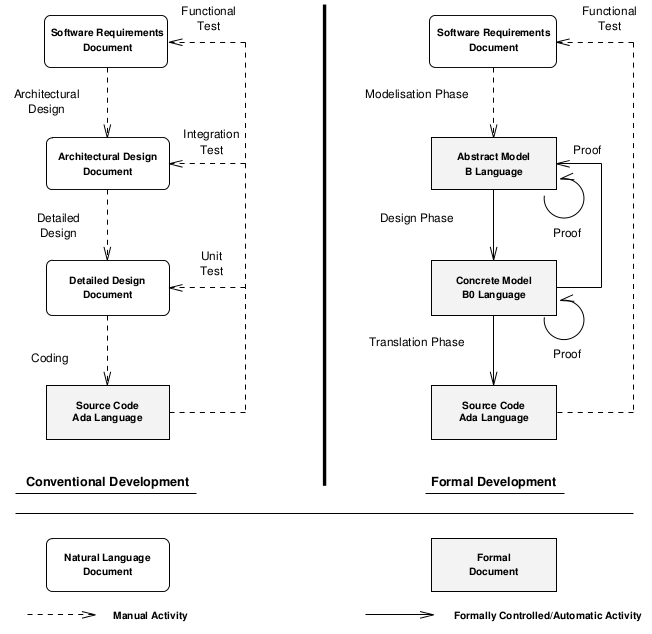
\includegraphics[scale=0.33]{ressources/formal_dev.png}
\end{figure}
\end{frame}

\iffalse
\section{Preuve de propriétés}
\begin{frame}
\frametitle{Preuve de programmes}
Le système de preuve est basée sur la vérification que :
\begin{itemize}
\item Les propriétés invariantes sont vérifiées par la
dynamique
\item Les raffinements préservent la correction totale
des propriétés invariantes
\end{itemize}

\pause
Pour cela, on se base sur la logique de Hoare :
\begin{itemize}
\item
Principe de correction partielle : $ \{P\}\;S\;\{Q\} $ 

Si l'état satisfait P avant S et si S termine, alors l'état satisfait Q après l'exécution de S.
\item
Recherche de la plus faible précondition:

Si l'état satisfait wp(S, Q) avant S alors S termine et l'état satisfait Q après.
On le note sous la forme de la substitution $[S]Q$.
\end{itemize}
\end{frame}

\begin{frame}
En résumé, le processus de raffinage consiste à :
\begin{itemize}
\item réduire l'indéterminisme
\item affaiblir les préconditions
\item renforcer les gardes
\item s'approcher de la machine concrète avec introduction u séquencement et de la boucle
on prouve que le raffinage se fait en respectant les fonctionnalités
\end{itemize}
\end{frame}
\fi

\iffalse
\subsection{Raffinement}
\begin{frame}
\frametitle{Obligations de preuve}
\begin{columns}[t]
  \begin{column}{5cm}
    \textsc{machine} $M$ \\
    \textsc{variables} $x$ \\
    \textsc{invariant} $I$ \\
    \textsc{initialisation} $U$ \\
    \textsc{operations} \\
    \quad $r \longleftarrow nom\_op(w) =$ \\
    \qquad \textsc{pre} $P$ \textsc{then} $K$ \textsc{end} \\
    \textsc{end}
\end{column}
  
  \begin{column}{5cm}
    \textsc{refinement} $N$ \textsc{refines} $M$ \\
    \textsc{variables} $y$ \\
    \textsc{invariant} $J$ \\
    \textsc{initialisation} $V$ \\
    \textsc{operations} \\
    \quad $r \longleftarrow nom\_op(w) =$ \\
    \qquad \textsc{pre} $Q$ \textsc{then} $L$ \textsc{end} \\
    \textsc{end}  
  \end{column}
\end{columns}  
 
Pour chaque opération il faut prouver:
\begin{itemize}
\item I ∧ J ∧ P ⇒ Q 
\item 
\end{itemize}
\end{frame}
\fi

\section{Diffusion de la méthode B}
\begin{frame}
\frametitle{Diffusion de la méthode B}
\framesubtitle{Météor}
Logiciel sécuritaire : 86 000 lignes Ada (1 000
composants)
\begin{itemize}
\item 115 000 lignes B
\item 27 800 obligations de preuve
\begin{itemize}
\item 81\% de preuve automatique
\item 92\% après ajout de règles (550)
\item 2 254 à prouver interactivement
\end{itemize}
\item Utilisateur d'un matériel sûr Vital Coded Processor (VCP) : processeur vérifiant son état et l'intégrité du code exécuté
\end{itemize}
\end{frame}

\begin{frame}
\frametitle{La méthode B événementielle}
\framesubtitle{Pour aller plus loin}
\begin{itemize}
\item Une machine en B  événementiel, n'a pas des opérations qui seront appelées par d'autres opérations, mais des  événements.
\item Un  événement est spécifié comme une opération gardée.
\end{itemize}

\end{frame}

\begin{frame}
\frametitle{Des questions ?}

\end{frame}
\end{document}
